
\section{Preliminary Results}


\begin{frame}
    \frametitle{Model Specification I}
    
Data: Standard and Poor’s (S\&P) 500 index retrieved from the \cite{SP500}.

\vspace{2mm}

    \begin{itemize}
    \item ARIMA(1,1,1) model 
        \begin{equation*}
        log(y_t) = c + log(y_{t-1}) + \phi_1\big[log(y_{t-1})-log(y_{t-2})\big] + \epsilon_t + \theta_1\epsilon_{t-1}
        \end{equation*}
    \item ETS(M,N,N) model
        \begin{align*}
        y_t &= \ell_{t-1} (1+\epsilon_t) \\
        \ell_t &= \ell_{t-1} (1+\alpha \epsilon_t) \\
        \end{align*}
        \vspace{-1cm}
    \item ETS(M,A,N) model
        \begin{align*}
        y_t &= (\ell_{t-1} + b_{t-1} (1+\epsilon_t) \\
        \ell_t &= (\ell_{t-1} + b_{t-1}) (1+\alpha \epsilon_t) \\
        b_t &= b_{t-1} + \beta (\ell_{t-1} + b_{t-1})\epsilon_t \\
        \end{align*}
    \end{itemize}

\end{frame}

\begin{frame}
    \frametitle{Model Specification II}

    \begin{itemize}
    \item A linear regression model of the S\&P 500 with a trend regressor and errors follow an ARIMA(1,0,0) process. 
        \begin{align*}
        y_t &= \beta_0 + \beta_1 t + u_t \\
        u_t &= \phi_1 \epsilon_{t-1} + \epsilon_t
        \end{align*}

    \item A linear regression model of the natural logarithm of S\&P 500 with a trend regressor and errors follow an ARIMA(1,0,0) process. 
        \begin{align*}
        log(y_t) &= \beta_0 + \beta_1 t + u_t \\
        u_t &= \phi_1 \epsilon_{t-1} + \epsilon_t
        \end{align*}
    \end{itemize}

Error terms $\epsilon_t$ in each model are assumed to be independent and normally distributed with a zero mean and a constant variance.

\end{frame}



\begin{frame}
    \frametitle{Ten sets of two-model pools}

\begin{table}[ht]
  \centering
  \small
  \caption{Log predictive score of density forecasts combination under two-model pools}
  \scalebox{0.80}{
    \begin{tabular}{llllll}
    \toprule
          & ARIMA(1,1,1) & ETS(M,N,N) & ETS(M,A,N) &  LM (linear) &  LM (log) \\
    \midrule
    ARIMA(1,1,1) & \textit{-5911.1974} & -5839.3045 & -5842.7634 & -5911.1974 & -5894.1267 \\
    ETS(M,N,N) & 0.45  & \textit{-5883.9697} & -5881.7790 & -5883.9697 & -5858.6397 \\
    ETS(M,A,N) & 0.43  & 0.08  & \textit{-5881.7970} & -5881.7970 & -5859.7980 \\
     LM (linear) & 1     & 1     & 1     & \textit{-7532.1464} & -5918.5230 \\
     LM (log) & 0.56  & 0.65  & 0.67  & 0     & \textit{-5918.5230} \\
    \bottomrule
    \multicolumn{6}{l}{\footnotesize The diagonal entries contains individual log score.}\\
    \multicolumn{6}{l}{\footnotesize The log scores for combination pools are located above the diagonal.}\\
    \multicolumn{6}{l}{\footnotesize Entries below the diagonal show the estimated weight of the model in that column.}\\
    \end{tabular}
    }
  \label{tab:2}
\end{table}

\end{frame}




\begin{frame}
    \frametitle{Top 4 Combinations}

\begin{figure}[ht]
\centering
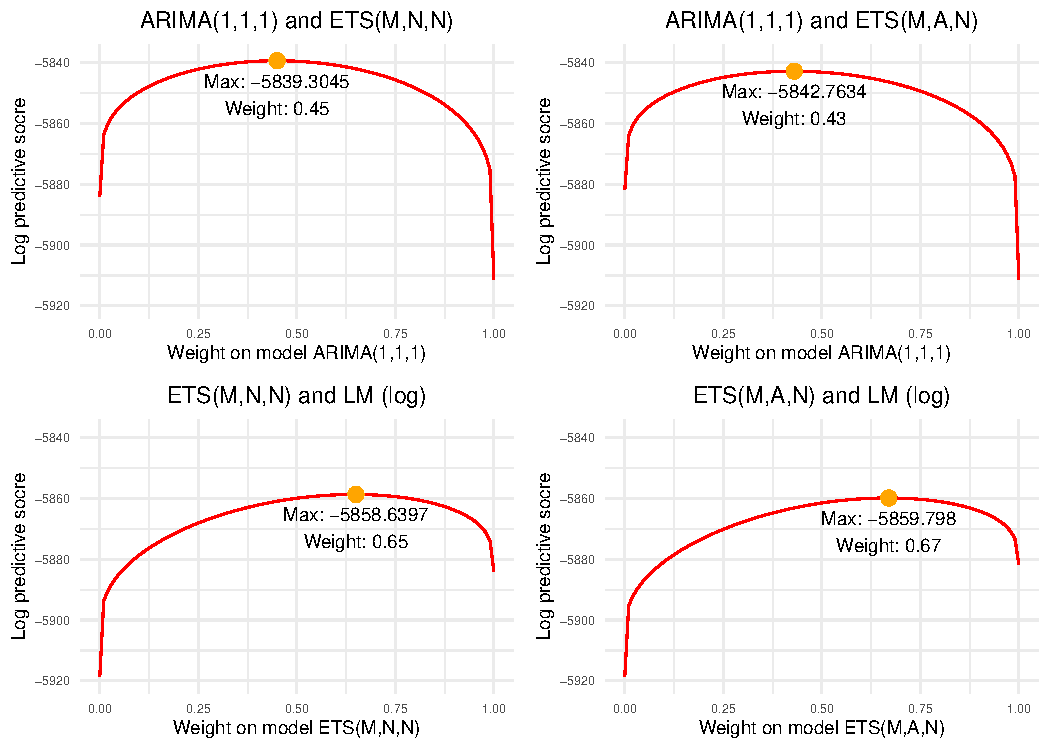
\includegraphics[width=9cm]{Graph/best4comb.pdf}\\
{\tiny{The top four log predictive scores of weighted two-model-pool combinations for S\&P 500 returns.}}
\end{figure}

\end{frame}


